\section{Task 1: QR decomposition}

\subsection{Method overview and problem}

QR decomposition factors a matrix \( A \) into a product of two matrices:
\[
A = QR,
\]
where:
\begin{itemize}
    \item \( Q \) is orthogonal (\( Q^T Q = I \)),
    \item \( R \) is upper triangular.
\end{itemize}

The decomposition uses the Gram--Schmidt process to orthogonalize the columns of \( A \). It can be written as:
\[
q_1 = \frac{a_1}{||a_1||}, \quad 
q_k = \frac{a_k - \sum_{i=1}^{k-1} \langle a_k, q_i \rangle q_i}{||a_k - \sum_{i=1}^{k-1} \langle a_k, q_i \rangle q_i||}.
\]

To assess accuracy, we measure the orthogonality error of \( Q \), defined as the largest inner product between distinct vectors \( q_i \) and \( q_j \), where \( i \neq j \):
\[
E = \max\{\langle q_i, q_j \rangle \; : \; i \neq j\}.
\]

Repeated QR decomposition can reduce orthogonality errors.

\subsection{Tests}

The tests examined orthogonality error versus matrix size \( n \) for two matrix types, taking the maximum inner product between different columns:
\begin{itemize}
    \item random matrices,
    \item diagonally dominant matrices.
\end{itemize}

The effect of a second QR decomposition on reducing orthogonality error was also analyzed. Matrix sizes ranged from \( n = 1 \) to \( n = 250 \). For each \( n \), 10 random matrices were generated and results were averaged.

\begin{minipage}{0.45\textwidth}
    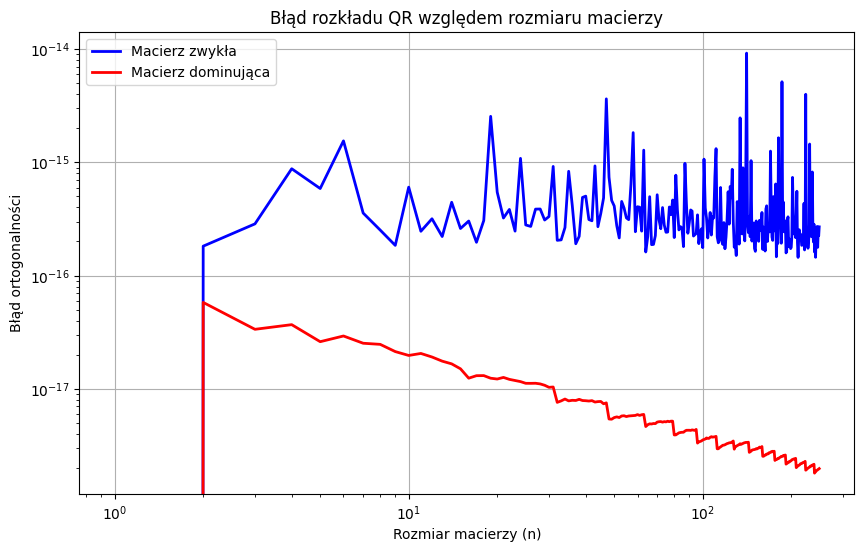
\includegraphics[width=\textwidth]{figures/task-1/error_size.png}
\end{minipage}
\hfill
\begin{minipage}{0.45\textwidth}
    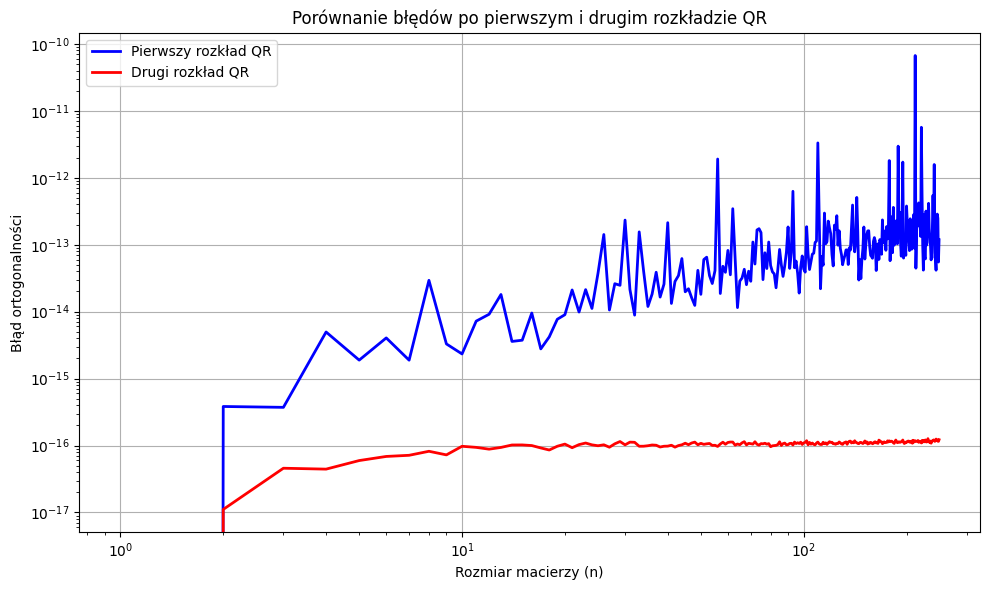
\includegraphics[width=\textwidth]{figures/task-1/second_QR.png}
\end{minipage}

\subsection{Results and analysis}
\begin{itemize}
    \item Orthogonality error depends differently on matrix size \( n \) for random and diagonally dominant matrices.
    \item A second QR decomposition substantially reduces orthogonality errors, as shown in the plot.
\end{itemize}

\subsection{Conclusions}
\begin{itemize}
    \item Repeated QR decomposition can substantially reduce orthogonality errors, which matters in applications requiring high precision.
    \item Errors of order \( 10^{-14} \) are negligible for most applications, but demanding computations may require additional accuracy-improvement steps.
\end{itemize}
